\subsection{Eksperimenta protokols: OpenCV FAST GPU implementācijas ātrdarbība}\label{appx:test2}
\setcounter{table}{0} %Reset table counter for (sub)appendix
\setcounter{figure}{0} %Reset figure counter for (sub)appendix
Eksperimenta mērķis ir novērtēt OpenCV FAST implementāciju GPU platformai.
Šī implementācija ir izstrādāta izpildei ar OpenCL savietojamu 
programmatūras platformu un pavadošo ierīces draiveri. Eksperiments veikts
ar, vienīgo autora rīcībā esošo sistēmu, kurai ir GPU ar OpenCL atbalstu
(sk.~\ref{tbl:test1-dev}~tabulu).
\begin{table}[hb]\small
	\centering
	\caption{Izmantotās iekārtas aprīkojums.}
	\label{tbl:test2-dev}
	\vspace{4pt}
	\begin{tabular}{ll}
		\toprule
		\textbf{CPU} & AMD Phenom II X6 2.80~GHz\\
		\textbf{Video adapteris} & ATI Radeon HD~6670 \\
		\midrule
		\textbf{Operētājsistēma} & Linux 3.8.0 (Ubuntu)\\
		\textbf{Video draiveris} & \texttt{fglrx} 9.1.11\\
		\textbf{OpenCL nodrošinājums} & AMD APP SDK 2.9\\
		\bottomrule
	\end{tabular}
\end{table}

Par ieejas datiem tika izmantota ,,\termEn{bas-relief}'' attēlu kopa%
	\footnote{Pieejama no \url{http://www.edwardrosten.com/work/junk.tar}}
un uzstādītais jutības slieksnis $t$ visos testos bija 25.
Katram attēla un implementācijas pārim tika veikti 20 mērījumi.
Lielā datu apjoma dēļ (60 ieraksti) visa kopa netiek atspoguļota. Datu
apkopojums redzams \ref{tbl:test2-data}~tabulā, kurā parādīts katra kopas
attēla (20) mērījumu sērijas vidējā vērtība un standartnovirze.
Rezultāti arī vizualizēti \ref{fig:test2-data}~attēlā, kur,
ar novirzes stabiņu, papildus attēlots
mērījumu sērijas absolūtais labākais (zemākais) rezultāts ar novirzes stabiņu.
\begin{table}[hb]\footnotesize
	\centering
	\caption{Ātrdarbības rezultāti.}
	\label{tbl:test2-data}
	\vspace{4pt}
	\begin{tabular}{c*{6}{r}}
		\toprule
		\input{results2-t1.tbl_tex}
		\bottomrule
	\end{tabular}
	\begin{minipage}{0.5\linewidth}
		\noindent Apzīmējumi:\\
		$\bar{t_p}$ --- attēla vidējais apstrādes laiks (20 mērījumos)\\
		$\sigma$ --- mērījumu sērijas standartnovirze
	\end{minipage}
\end{table}

Rezultātos var novērot, ka FAST GPU implementācijas ātrdarbība ir līdzīga
CPU implementācijām, bet to nepārsniedz. Autors šo veiktspējas
ierobežojumu skaidro ar salīdzinoši mazo datu apjomu un
zemu nepieciešamo skaitļošanas apjomu. Tādējādi GPU straumes
procesori nav pietiekami piesātināti ar datiem, kā rezultātā tie
procentuāli daudz laika pavada dīkstāvē un
GPU augstais latentums ir galvenais ierobežojošais faktors.
%~ (GPU arhitektūra apskatīta \ref{sec:gpu}~nodaļā).

Autors novēro, ka OpenCV FAST GPU implementācija balstās uz
\termEn{integer} tipa aritmētiku, kas nav tik efektīva, kā
peldošā komata skaitļu aritmētika, GPU platformām, bet, ņemot vērā
iepriekš secināto, uzskata, ka aritmētikas tipa izvēle neatstāj nekādu
būtisku iespaidu uz veiktspēju šajā gadījumā.

\begin{figure}[t]
	\centering
	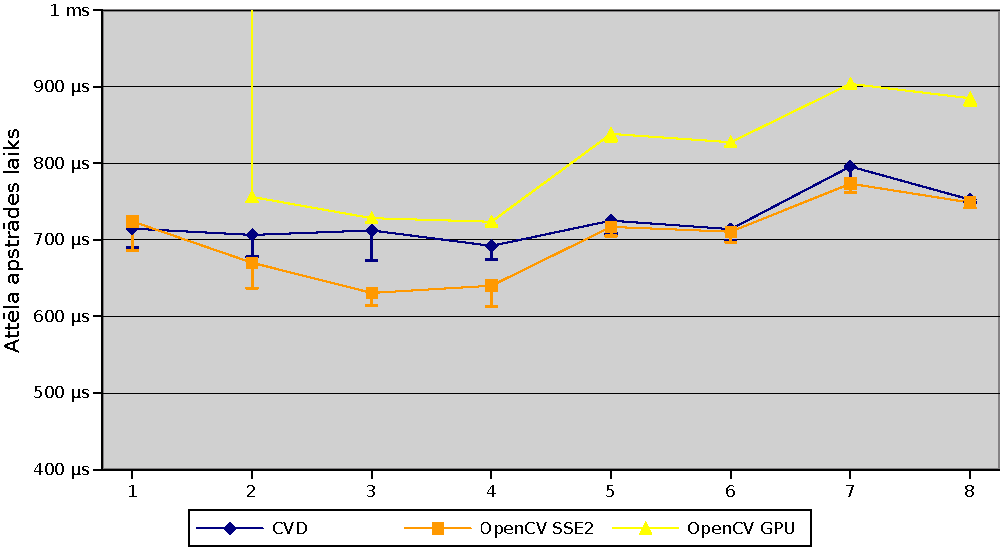
\includegraphics[scale=0.77]{chart-gpu}
	\caption{Attēlu vidējais apstrādes laiks $\bar{t_p}$ dažādiem attēliem.}
	\label{fig:test2-data}
\end{figure}
Mērījumos arī var novērot ļoti augstu apstrādes laiku pirmajam attēlam. Tas
skaidrojams ar to, ka OpenCL kods tiek mērķa ierīcei kompilēts izpildes
laikā. 
Papildus novērojama mazāka standartnovirze GPU implementācijas mērījumiem,
salīdzinot ar CPU implementācijām, jo CPU gadījumā skaitļošanas laiku
izmanto arī operētājsistēma un citas lietojumprogrammas, bet GPU resursi
tiek rezervēti uzdevuma izpildei.
\begin{figure}[bh]
	\centering
	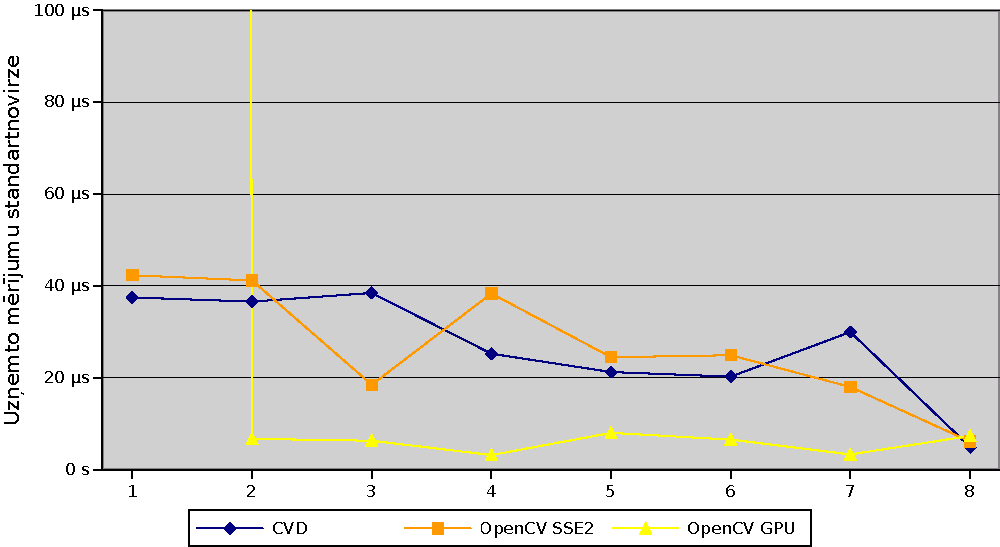
\includegraphics[scale=0.77]{chart-gpu-stdev}
	\caption{Attēlu apstrādes laiku standartnovirze}
	\label{fig:test2-stdev}
\end{figure}
